\documentclass[11pt,letterpaper]{article}
\usepackage[lmargin=1in,rmargin=1in,bmargin=1in,tmargin=1in]{geometry}
\usepackage{checkins}

\pgfplotsset{soldot/.style={color=black,only marks,mark=*},
		holdot/.style={color=black,fill=white,only marks,mark=*},
		compat=1.12
}

% -------------------
% Content
% -------------------
\begin{document}
\thispagestyle{title}

% 01/15
\checkin{01/15} \textit{True/False}: If $f(3)= 5$, then $\ds\lim_{x \to 3} f(x)= 5$. \pspace

\sol The statement is \textit{false}. Recall that the limit of a function (if it exists) is what the output gets `close' to as the input gets `close' to its limiting value. The fact that $f(3)= 5$ does not mean the outputs are all `close' to 5 when $x$ is `close' to 3. For instance, consider the function $f(x)$ plotted below.
	\[
	\fbox{%
	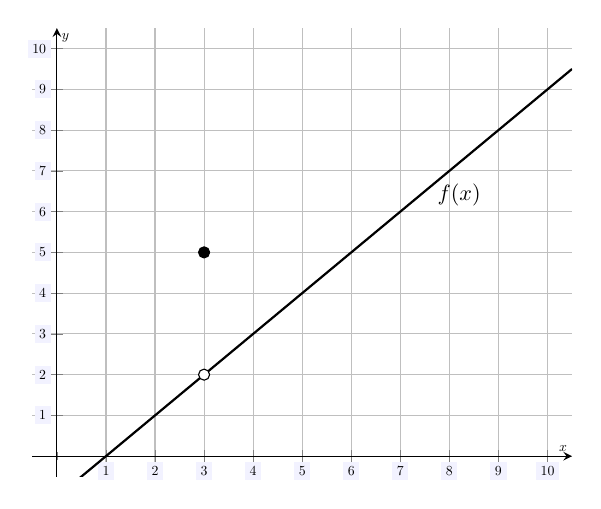
\begin{tikzpicture}[scale=1,every node/.style={scale=0.5}]
	\begin{axis}[
	grid=both,
	axis lines=middle,
	ticklabel style={fill=blue!5!white},
	xmin= -0.5, xmax=10.5,
	ymin= -0.5, ymax=10.5,
	xtick={-1,0,...,11},
	ytick={-1,0,...,11},
	minor tick = {-11,-10,...,11},
	xlabel=\(x\),ylabel=\(y\),
	samples=20]
	\node at (8.2,6.4) {\scalebox{1.6}{$f(x)$}};
	\addplot[thick, samples=5, domain= -0.5:10.5] {x - 1};
	\addplot[soldot] coordinates{(3,5)};
	\addplot[holdot] coordinates{(3,2)};
	\end{axis}
	\end{tikzpicture}
	}
	\]
Despite the fact that $f(3)= 5$, $\ds\lim_{x \to 3} f(x)= 2$ because all the outputs are `close' to 2 when the inputs are `close' to 3. \pvspace{1.3cm}



% 01/17
\checkin{01/17} \textit{True/False}: Let $f(x)$ be a function defined on all real numbers such that $\ds\lim_{x \to \pi} f(x)= 10$. Then it must be that $\ds\lim_{x \to \pi^+} f(x)= 10$. \pspace

\sol The statement is \textit{true}. Recall that the limit (if it exists) is what the output gets `close' to as the input gets `close' to its limiting value. Because $\ds\lim_{x \to \pi} f(x)= 10$, the outputs of $f(x)$ are all `close' to 10 whenever $x$ is `close' to $\pi$---no matter how $x$ is `close' to $\pi$. The right-hand limit $\ds\lim_{x \to \pi^+} f(x)$ asks what the outputs are `close' to if $x$ is `close' to $\pi$---but bigger than $\pi$. But we already know that the outputs are `close' to 10. Therefore, it must be that $\ds\lim_{x \to \pi^+} f(x)= 10$. Recall that $\ds\lim_{x \to a} f(x)= L$ if and only if $\lim_{x \to a^-} f(x)= L$ and $\lim_{x \to a^+} f(x)= L$. \pvspace{1.3cm}



% 01/22
\checkin{01/22} $\ds\lim_{x \to \infty} \left(1 + \dfrac{1}{3x} \right)^x= e^3$ \pspace

\sol The statement is \textit{false}. Recall that $\ds\lim_{x \to \infty} \left(1 + \dfrac{1}{x} \right)^x= e$. But then\dots
	\[
	\lim_{x \to \infty} \left(1 + \dfrac{1}{3x} \right)^x= \lim_{x \to \infty} \left(1 + \dfrac{1}{3x} \right)^{x \cdot 3/3}= \lim_{x \to \infty} \left[ \left(1 + \dfrac{1}{3x} \right)^{3x} \right]^{1/3}= e^{1/3}= \sqrt[3]{e}
	\] \pvspace{1.3cm}



% 01/24
\checkin{01/24} $\ds\lim_{x \to \infty} \left(1 + \dfrac{1}{x} \right)^x= \left(1 + 0\right)^\infty= 1^\infty= 1$ \pspace

\sol The statement is \textit{false}. One does obtain $1^\infty$ after na\"ively plugging in $x= \infty$. However, $\infty$ is not a number; moreover, although one might feel otherwise, it is simply need not be the case that $1^\infty= 1$. Indeed, $1^\infty$ is an indeterminant form. One could correctly recall that\dots
	\[
	\lim_{x \to \infty} \left(1 + \dfrac{1}{x} \right)^x= e
	\] \pvspace{1.3cm}



% 01/27
\checkin{01/27} The function $f(x)= \dfrac{e^x \sin(\sqrt[3]{x})}{x^2 + 6x + 9}$ is continuous on any interval which does not contain $x= -3$. \pspace

\sol The statement is \textit{true}. We know that $e^x$, $\sin x$, $\sqrt[3]{x}$, and $x^2 + 6x + 9$ are everywhere continuous. But then $\sin(\sqrt[3]{x})$ is everywhere continuous, because it is a composition of continuous functions. This makes $e^x \sin(\sqrt[3]{x})$ continuous, because it is the product of continuous functions. But then $f(x)= \dfrac{e^x \sin(\sqrt[3]{x})}{x^2 + 6x + 9}$ is continuous so long as $x^2 + 6x + 9 \neq 0$, because it would be a quotient of continuous functions. Observe that $x^2 + 6x + 9= (x + 3)^2$. Therefore, if $x^2 + 6x + 9= 0$, then $(x + 3)^2= 0$ so that $x= -3$. Therefore, $f(x)$ is continuous on any interval not containing $-3$. \pvspace{1.3cm}



% 01/29
\checkin{01/29} The limit $\ds\lim_{x \to 0} \dfrac{\sqrt{x + 9} - 3}{x}$ represents $f'(9)$, where $f(x)= \sqrt{x}$. 

\sol The statement is \textit{true}. The definition of the derivative at $x= a$ is $\ds f'(a)= \lim_{h \to 0} \dfrac{f(a + h) - f(a)}{h}$. Taking $f(x)= \sqrt{x}$ and $a= 9$, we would have $\ds f'(9)= \lim_{h \to 0} \dfrac{f(9 + h) - f(9)}{h}= \lim_{h \to 0} \dfrac{\sqrt{9 + h} - \sqrt{9}}{h}= \lim_{h \to 0} \dfrac{\sqrt{h + 9} - 3}{h}$. This is the same as the given limit with the role of $h$ and $x$ interchanged. \pvspace{1.3cm}



% 01/31
\checkin{01/31} $\dfrac{d}{dx} \, \sin(\ln x)= \cos \left( \dfrac{1}{x} \right)$ \pspace

\sol The statement is \textit{false}. We have a derivative of a composition of functions. This requires chain rule: $\frac{d}{dx}\, f \big( g(x) \big)= f' \big( g(x) \big) \cdot g'(x)$. Here, we have $f(x)= \sin x$ and $g(x)= \ln x$. The correct derivative should be\dots
	\[
	\dfrac{d}{dx} \, \sin(\ln x)= \cos(\ln x) \cdot \dfrac{1}{x}
	\]
Here, the `rule' $\frac{d}{dx} f \big( g(x) \big)= f' \big( g'(x) \big)$ has been applied, which is incorrect. \pvspace{1.3cm}



\newpage



% 02/03
\checkin{02/03} $\dfrac{d}{dx} \; x^3 \sin(x)= 3x^2 \cos x$ \pspace

\sol The statement is \textit{incorrect}. We have a derivative of a product of functions. This requires the product rule: $\frac{d}{dx} f(x) g(x)= f'(x) g(x) + f(x) g'(x)$. Here, we have $f(x)= x^3$ and $g(x)= \sin x$. The correct derivative should be\dots
	\[
	\dfrac{d}{dx}\, x^3 \sin x= 3x^2 \cdot \sin x + x^3 \cdot \cos x
	\]
Here, the `rule' $\frac{d}{dx} f(x) g(x)= f'(x) g'(x)$ has been applied, which is incorrect. \pvspace{1.3cm}



% 02/05
\checkin{02/05} If $\theta_d$ is an angle measured in degrees, then $\dfrac{d}{d\theta}\, \sin(\theta_d)= \cos(\theta_d)$. \pspace

\sol The statement is \textit{false}. This is a problem which can arise in working with derivatives with `mixed units' or especially when programming computer systems to perform the computations and one is not paying attention to the units. Trigonometric functions should be computed using radians. Even if one wishes to use degrees, the units would need to be consistent. Clearly, $\frac{d}{d\theta}$ is the derivative with respect to $\theta$---measured in radians. However, the input to the trigonometric function is in degrees. We would need to convert this input to radians by multiplying by $\frac{\pi}{180}$. But then\dots
	\[
	\dfrac{d}{d\theta} \sin(\theta_d)= \dfrac{d}{d\theta} \sin \left(\theta \cdot \dfrac{\pi}{180} \right)= \dfrac{\pi}{180} \cdot \cos \left(\theta \cdot \dfrac{\pi}{180} \right)= \dfrac{\pi}{180} \cos \left( \theta_d \right)
	\]
One can work out the derivation of $\frac{d}{d\theta} \sin \theta$ to see the reliance on radians to get a deeper---non-chain rule---reason for why this is the case. \pvspace{1.3cm}



% 02/10
\checkin{02/10}
























\end{document}